%Started on 9th August 2006
%Aug: 11, 22, 23, 24, 25, 28, 29, 30, 31
%Sep:  1,  7,  8
% 2007
%Jan: 15, 16, 17, 22
%Feb:  1,  2,  4,  5,  6,  8,  9, 11, 22, 26
%Mar:  8, 12, 13, 16, 17, 20, 21, 22, 27, 28, 29, 30, 31
%Apr:  1,  2, 16, 18, 19, 21, 28, 29, 30
%May:  2,  4,  8, 11, 12, 13, 14
%Sep: 18, 19, 20, 27
%Oct:  1

%
% Chapter: Practical implementations of Interior point methods
%
\label{ch:PracticalIpm}

In this chapter we turn our attention to the computational side of
interior point methods. We concentrate on the main strategies which are
at the basis of effective implementations of interior point methods
for linear programming, and present other issues that are specific
to practical algorithms.
These have been documented extensively; for example, see
\cite{AndersenGondzioMeszarosXu,GondzioTerlaky,ipm:Wright97} 
and the references therein.
We also review some of the warm-start techniques for interior point methods
that have been proposed in the literature.


%
% Section
%
\section{Considerations for practical algorithms}

In Sections~\ref{sec:FeasibleMethods} and \ref{sec:InfeasibleMethods}
we presented theoretical
results on the order of convergence of some interior point algorithms.
In practice, convergence is much faster than stated by those results, as
optimality is usually reached in a number of iterations 
proportional to the logarithm of the problem dimension. 
This was also shown by Ye \cite[Chapter~6]{Ye97} through an
average-case and probabilistic analysis.
As in the analysis of the simplex method, we see here a large
gap between the predicted and observed performances that is still to
be fully understood.

Interior point methods are well-suited to solving very
large scale optimization problems.
Practical algorithms are very different from the ones used for
theoretical purposes, and they usually implement some variation
of infeasible interior point algorithms. In particular they show
differences in the computation of the search directions, 
the evaluation of the stepsize, 
the use of the neighbourhood concept, and the update of the
barrier parameter.
This is further complicated by issues of computational efficiency
and numerical stability, which often suggest the use of amended
techniques or heuristic approaches, which make
the analysis of the algorithms implemented in practice extremely difficult.

In the rest of this section we illustrate some of 
the algorithmic differences that are relevant to any 
practical implementation of interior point methods.
They concern the choice of the starting point, the techniques
used for solving the Newton system (\ref{eq:NewtonSystem}), the computation
of the stepsize, the termination criteria and the use
of correctors in the search directions.
This selection has been made according to the relevance
for this thesis.
We will therefore not discuss other topics of extreme importance 
in practical algorithms such as presolve techniques, 
detection of infeasibilities, linear algebra implementations, 
use of iterative methods in the solution of the Newton system,
and many others.
Valuable references for these additional topics can be found in
\cite{AndersenGondzioMeszarosXu,GondzioTerlaky}.

%
%
\subsection{Mehrotra's starting point heuristic}
\label{sec:StartingPoint}

The initialisation of an interior point method consists of two
logically independent steps: the presolve phase (in which some
heuristic strategies are employed in finding duplicate rows or
columns, discovering fixed variables, removing redundant constraints 
and tightening the bounds)
and the process of finding an initial iterate.
Here we discuss only the latter, and refer the reader 
to \cite{AndersenAndersen}
for a treatment of the important topic of presolve techniques.

The choice of an initial iterate for interior point methods is a
critical one. It challenges both the feasible and infeasible
algorithms, and the solutions proposed in the two contexts are
completely different.
For infeasible algorithms the major hurdle
of finding a feasible starting point is removed. 
However, the practical performance is very sensitive to the initial
iterate, so the use of arbitrary points is not recommended.
In particular, two requirements become important: the centrality 
of the point and the magnitude of the corresponding infeasibilities.

Mehrotra \cite{Mehrotra92} introduced a tool to find a starting point 
that attempts to fulfil the above requirements. In this
heuristic, we solve two least squares problems which aim to
satisfy the primal and dual constraints:
\begin{eqnarray*}
  \min_x      \!\! & x^Tx & \;\;\mbox{s.t. }\; Ax = b,      \\
  \min_{(y,s)}\!\! & s^Ts & \;\;\mbox{s.t. }\; A^Ty + s = c.
\end{eqnarray*}
These problems have solution
\[
  \tilde x = A^T(AA^T)^{-1}b, \quad
  \tilde y = (AA^T)^{-1}Ac, \quad
  \tilde s = c - A^T \tilde y.
\]
The solution $\tilde w$ is further 
shifted inside the positive orthant, and the starting point is
\[
  w^0 = (\tilde x + \delta_x e,\, \tilde y,\, \tilde s + \delta_s e),
\]
where $\delta_x$ and $\delta_s$ are positive quantities. 
Their values depend on the distance of $\tilde x$ and $\tilde s$
to non-negativity and an additional correction term to ensure
strict positivity.

The following variation is described in \cite{GondzioTerlaky}:
\begin{eqnarray*} 
  \min_x      \!\! & c^Tx + \rho x^Tx & \;\;\mbox{s.t. }\; Ax = b,      \\
  \min_{(y,s)}\!\! & b^Ty + \rho s^Ts & \;\;\mbox{s.t. }\; A^Ty + s = c,
\end{eqnarray*}
where the parameter $\rho$ is fixed to a predetermined value, in order
to compensate for the contribution of the primal and dual objectives.

Mehrotra's starting point strategy has some drawbacks. It is scale dependent,
it is affected by the presence of redundant constraints,
and it does not guarantee producing a well-centered iterate.
However it is commonly employed in interior point codes, and it is
considered to be an effective heuristic for determining a starting point.

Considerations on what constitutes an appropriate starting point 
for interior point methods will be discussed
again in Section~\ref{sec:WarmStart}, where we survey some
warm-start strategies.

%
%
\subsection{Computation of the stepsize}

The computation of different stepsizes in the primal and dual spaces is
done almost universally in implementations of interior point methods
for linear programming.
% (while for quadratic programs the stepsizes have to be identical). 
This has the advantage of
speeding up the restoration of feasibility. According to
\cite{GondzioTerlaky}, the use of different stepsizes contributes 
to a reduction of 10\% in the number of iterations required 
when solving the Netlib 
set of tests.

In order to ensure that the $(x,s)$ components of the iterate
remain positive after moving along the
$\Delta w$ direction, we need to employ a linesearch procedure 
and find the maximum feasible stepsizes $\alpha_P$ and $\alpha_D$ 
such that
\[
  x + \alpha_P \Delta x > 0, \qquad  s + \alpha_D \Delta s > 0.
\]
The achievable stepsizes for a given search direction $\Delta w$, 
in the primal and dual space respectively, are computed as:
\be  \label{eq:Alphas}
  \alpha_P =\min \left\{ -\frac{x_i}{\Delta x_i} : \Delta x_i < 0 \right\},
  \quad\;
  \alpha_D =\min \left\{ -\frac{s_i}{\Delta s_i} : \Delta s_i < 0 \right\}.
\ee
These stepsizes are then shortened with a factor $\alpha_0 = 0.99995$
to ensure strict positivity \cite{GondzioTerlaky,LustigMarstenShanno}.

We remark that in the computation of the stepsizes, we 
maintain the strict positivity of the iterates, without restricting
the point inside a neighbourhood.
While this is done on the grounds of computational efficiency, we may
lose the global convergence property ensured by keeping the
iterates in a neighbourhood of the central path.

%
%
\subsection{Termination criteria}

In contrast to active set algorithms, interior point methods reach a
solution only asymptotically. 
Because of the presence of the barrier term that keeps the iterates
away from the boundary, they can never produce an exact solution.
When working in the context of limited precision of the
floating point representation typical of computers, feasibility and
complementarity can be attained only within a certain level
of accuracy.

For these reasons, criteria have to be established according
to which the termination of the algorithm can be decided.
Some common termination criteria used in practice are the
following \cite{GondzioTerlaky}:
\be  \label{eq:TerminationCriteria}
\frac{\| Ax - b \|}{1 + \|x\|_\infty} \le10 ^{-p}, 
\qquad
\frac{\| A^Ty + s - c \|}{1 + \|s\|_\infty} \le10 ^{-p},
\qquad
\frac{| c^Tx - b^Ty |}{1 + | b^Ty |} \le10 ^{-q}.
\ee
The values of $p$ and $q$ required depend on the specific application.
In the literature, it is common to use the value $p = q = 8$.

Another set of criteria, implemented in the interior point code
\PCx \cite{PCx} is given by:
\be  \label{eq:TerminationCriteriaPCx}
\frac{\| Ax - b \|}{1 + \|b\|} \le 10^{-p},
\qquad
\frac{\| A^Ty + s - c \|}{1 + \|c\|} \le 10^{-p},
\qquad
\frac{\mu}{1 + |c^T x|} \le 10^{-q}.
\ee
The last condition in \eqref{eq:TerminationCriteriaPCx} is weaker
than the corresponding one in \eqref{eq:TerminationCriteria} as,
through $\mu$, it depends on $n$. Therefore, in this case it is common to 
require $q = 10$.

The third condition in each set is usually the most important, as it is
commonly attained only after the feasibility requirements are satisfied.
It is worth noting that the criteria (\ref{eq:TerminationCriteria})
and (\ref{eq:TerminationCriteriaPCx})
are dependent on the scaling of the data.

Once a solution has been found within a prescribed 
optimality tolerance, such a point can be projected onto a face 
of the polyhedron in an efficient way.
This can be done using a strongly polynomial algorithm due
to Megiddo \cite{Megiddo91}. This procedure goes under the name
of {\em basis crossover}, 
as, given a complementary primal--dual solution, it generates a basis 
that is both primal and dual feasible.

%
%
\subsection{Solving the Newton system}
\label{sec:SolvingNewtonSystem}

The solution of system (\ref{eq:NewtonSystem}) is the computationally
dominant step in each iteration of an interior point algorithm.
Throughout this thesis, we will 
restrict our attention to using a direct approach in solving these
equations.
We remark, however, that a wealth of research has explored the use
of iterative methods in the computation of the search direction
\cite{BergamaschiGondzioZilli,OliveiraSorensen05}.

System (\ref{eq:NewtonSystem}) is usually reduced to two other
formulations by exploiting the block structure of its
matrix.
%
The {\em augmented system} formulation is obtained by using 
the last row of (\ref{eq:NewtonSystem}) to eliminate
$\Delta s = X^{-1} (\xi_\mu - S\Delta x)$.
This produces
%
\be \label{eq:AugmentedSystem}
\left[ \begin{array}{cc}
    -X^{-1}S & A^T \\ A & 0
  \end{array} \right]
\left[ \begin{array}{c}
    \Delta x \\  \Delta y
  \end{array} \right] =
\left[ \begin{array}{c}
    \xi_c - X^{-1}\xi_\mu \\ \xi_b
   \end{array} \right],
\ee
which is a symmetric but indefinite system.
%
By further eliminating $\Delta x$, we reduce system 
(\ref{eq:AugmentedSystem}) to the set of {\em normal equations}
%
\be \label{eq:NormalEquations}
  A D^2 A^T \Delta y = A D^2 (\xi_c - X^{-1} \xi_\mu) + \xi_b,
\ee
%
where we introduced the notation $D^2 = S^{-1} X$.
Under the standard assumption of full row rank for $A$, matrix 
$A D^2 A^T$ is positive definite, since $D^2_i = x_i/s_i > 0$ for
all $i = 1, \ldots, n$.

Besides the issue of definiteness, the two formulations differ in
terms of sparsity and conditioning, the normal equations usually 
being denser and worse conditioned.
The choice between the augmented system and normal equations
techniques depends also on 
the relative density of $AD^2A^T$ with respect to $A$.

Normal equations are to be avoided when there are dense columns in $A$, 
as they generate dense blocks in $AD^2A^T$.
In the broad context of weighted least squares computations, the choice
between the augmented system and normal equations techniques was studied long
before the development of interior point methods, see for example
\cite{DuffErismanReid86}.

The augmented system formulation requires particular attention 
to the development of linear algebra routines because
it involves an indefinite matrix. This raises problems of numerical
stability, and an accurate choice of pivoting strategies is fundamental.
Maros and M\'esz\'aros \cite{MarosMeszaros} presented an in-depth 
study of the properties of the augmented system formulation.

A direct approach computes the Cholesky factorisation $M=LDL^T$
of the constraint matrix $M$ with a lower triangular $L$ and
a diagonal matrix $D$.
In the computation of the factors, inevitably new nonzero entries
are generated (the so called {\em fill-in}). The amount of
fill-in is strongly influenced by the ordering in which the
operations are performed.
Various ordering techniques have been developed to reduce the fill-in
in the Cholesky factors, thus maintaining sparsity and 
reducing the required work \cite{RothbergHendrickson}.
Once the factors have been computed, the solution of system $Mx = r$ 
happens in two steps:
first by solving $Lz = r$ for $z$, then $L^Tx = D^{-1}z$ for $x$.
The solution phase is also called the {\em backsolve phase}.
A careful implementation of the linear algebra routines that perform
the ordering, factorisation and solution of the Newton system is
one of the key points for an efficient interior point solver.

The computation of the Cholesky factors
dominates the cost of each iteration.
As this is usually a major computational task, 
the efforts in the theory and practice of 
interior point methods concentrate on reducing 
the number of times the Newton system matrix (\ref{eq:NewtonSystem}) 
has to be factorised.
In particular, it is worth adding more (cheap) 
backsolves if this reduces the number of (expensive) factorisations. 

Two techniques have proved particularly successful in reducing 
the number of iterations within practical algorithms:
Mehrotra's predictor--corrector algorithm \cite{Mehrotra92} 
and multiple centrality correctors \cite{Gondzio96}. 
Mehrotra's predictor--corrector technique \cite{Mehrotra92} uses two 
backsolves per factorisation; the multiple centrality correctors technique
\cite{Gondzio96} allows recursive corrections. A larger number 
of backsolves per iteration is allowed, leading to a further reduction 
in the overall number of factorisations. 
These 
techniques have been implemented in most commercial and academic 
interior point solvers for linear and quadratic programming such 
as {\sc bpmpd}, Cplex, \HOPDM, Mosek, Ipopt, \OOPS, {\sc ooqp}, \PCx and Xpress
(see Appendix B in \cite{ipm:Wright97}).

Since these two methods were developed, there have been a number of 
attempts to investigate their behaviour rigorously and thus provide
further insight on their success. 
Such objectives are difficult to achieve because 
correctors use heuristics that are effective in practice but hard 
to analyse theoretically. 
Besides, both correcting techniques are applied to long-step and infeasible 
algorithms which have very little in common with the short-step and 
feasible algorithms that display the best known theoretical complexity.
These strategies will be the focus of the next two sections.


%
% Section
%
\section{Mehrotra's predictor--corrector algorithm}
\label{sec:MehrotraPC}

In Mehrotra's predictor--corrector algorithm \cite{Mehrotra92}, 
first a predictor direction is generated 
to make progress towards optimality, and then 
a corrector is computed to remedy for some of the error made by the predictor
and move the iterate closer to the central path.

A number of advantages can be obtained by exploiting the
linearity in the Newton system (\ref{eq:NewtonSystem}) and
considering the right-hand as
\[
 \left[ 
  \begin{array}{c}
    b-Ax \\ c-A^Ty-s \\ -XSe + \sigma\mu e
  \end{array} \right]
 = \left[ 
  \begin{array}{c}
    b-Ax \\ c-A^Ty-s \\ -XSe
  \end{array} \right]
 + \left[ 
  \begin{array}{c}
    0 \\ 0 \\ \sigma\mu e
  \end{array} \right],
\]
thus splitting the computation 
of the Newton direction into two steps, corresponding to solving the linear
system (\ref{eq:NewtonSystem}) independently for the two right-hand 
sides above.

First, we can postpone the choice of the centering parameter 
$\sigma$ and base it on the assessment of the quality of the 
pure Newton direction computed with the first part of the right-hand side;
second, the error made by this direction may be 
taken into account and
corrected. Mehrotra's predictor--corrector algorithm \cite{Mehrotra92}
translates these observations into a powerful computational method.
This technique
is extremely efficient in practice \cite{LustigMarstenShanno,Mehrotra92}. 
Since its introduction, it has 
been considered the method of choice for practical implementations 
because it is usually very fast and reliable. Moreover, it has a 
convincing interpretation in terms of second-order approximations
to the central path.

%
%
\subsection{Affine-scaling predictor direction}

The {\em predictor direction} 
$\Delta_a w = (\Delta_a x, \Delta_a y, \Delta_a s)$ is obtained by solving 
system (\ref{eq:NewtonSystem}) with right-hand side 
\be  \label{eq:PredictorRhs}
 r_a = \left[ 
  \begin{array}{c}
    b-Ax \\ c-A^Ty-s \\ -XSe
  \end{array} \right].
\ee
This corresponds to computing the pure Newton direction for the
original \KKT system (\ref{eq:KKT}), and this direction is often
called the {\em affine-scaling} direction. This 
direction optimizes strongly, as it targets a point for which 
all complementarity products are zero. 
The achievable stepsizes for the predictor direction, 
in the primal and dual space respectively, are computed 
according to (\ref{eq:Alphas}).

As it targets a point for which $XSe = 0$, the affine-scaling direction 
may be distracted by points that have small complementarity products 
but are not optimal. 
In particular, it may well point towards the boundary of the 
positive orthant or approach an infeasible vertex, generating 
a very small stepsize. 
This effect is usually worsened if the current iterate is badly centered, 
and therefore only a very small step is acceptable in order to 
maintain positivity or to keep the iterate in some neighbourhood 
of the central path.

Since it completely ignores the central path, the affine-scaling 
direction is not enough in a practical implementation of 
interior point methods, but has to be 
complemented by other techniques.
The role of the centering term is to remedy this situation by 
causing the search direction to rotate towards the interior 
of the feasible region,
therefore allowing a longer stepsize. 
Tapia \etal \cite{TapiaZhangSaltzmanWeiser} noted that the choice of the 
centering parameter can be crucial both in theory and in practice,
and suggest that it is a function of the Newton step. 
This calls for two separate backsolves at each iteration.

%
%
\subsection{Second-order corrector direction}

Mehrotra's algorithm exploits a centrality corrector in order to 
remedy badly centered points. The purpose of this direction is 
to move closer to the central path, and therefore reduce the spread 
in complementarity products, without aiming for more optimality. 
This is a somewhat conservative direction, which it is hoped will 
provide more room for movement at the next iteration.

One tool introduced by Mehrotra \cite{Mehrotra92} is a dynamic evaluation 
of the centering parameter $\sigma$. It is based on a simple  
heuristic that evaluates the quality of the predictor direction
in order to judge the amount of centering term needed.
%
The length of the feasible steps $\alpha_P$ and $\alpha_D$
for the affine-scaling direction are used to 
predict the complementarity gap after such a step:
\be \label{eq:PredictedGap}
  g_a = (x + \alpha_P \Delta_a x)^T(s + \alpha_D \Delta_a s).
\ee

The ratio $g_a / x^{T}s \in (0,1)$ measures the quality of the 
predictor direction.
A small ratio indicates a successful reduction of the complementarity 
gap. On the other hand, if the ratio is close to one, then very little 
progress is achievable along the direction $\Delta_a w$,
and a bigger centering term
is recommended.

In \cite{Mehrotra92} the following choice of the new barrier parameter 
is suggested
%
\be \label{eq:Mu}
  \left( \frac{g_a}{x^{T}s} \right)^{\! 2} \, \frac{g_a}{n}
           = \left( \frac{g_a}{x^{T}s} \right)^{\! 3} \, \frac{x^{T}s}{n},
\ee
%
corresponding to the choice of $\sigma = (g_a / x^Ts)^3$ 
for the centering parameter. 
If the predictor provides a good improvement, a small $\sigma$ 
is chosen, and very little centering will be used. When, 
on the other hand, the affine-scaling direction produces very small stepsizes 
and very little improvement can be achieved, $\sigma$ will be 
close to one, and a stronger recentering will occur.

The centering parameter, could be chosen more generally as
\[
  \sigma = \left( \frac{g_a}{x^Ts} \right)^p\!\!,
\]
for various choices of the exponent $p$. Mehrotra \cite{Mehrotra92}
studied the effect of different values $p=1,2,3,4$
on a subset of Netlib problems, and concluded that for $p$ between
2 and 4 there was not much difference.
Also Lustig \etal \cite{LustigMarstenShanno} commented on the
weak dependence of the computational performance on the choice 
of the exponent, and settled for the value $p=2$.

A further important contribution by Mehrotra is the 
introduction of a second-order direction. 
As said above, the affine-scaling direction 
corresponds to a linear approximation to the the trajectory from 
the current point to the optimal set, where no information about 
higher-order terms is taken into account. This linearisation, 
however, produces an error which can be determined analytically.
%
Assuming that a full step in the affine-scaling direction is made, 
the new complementarity products are equal to
\[
  (X + \Delta_a X) (S + \Delta_a S) e 
   \;=\; XSe + (S \Delta_a x + X \Delta_a s) + \Delta_a X \Delta_a S e
   \;=\; \Delta_a X \Delta_a S e,
\]
as the third equation in the Newton system (\ref{eq:NewtonSystem}) satisfies 
$S \Delta_a x + X \Delta_a s = -XSe.$
%
The term $\Delta_a X \Delta_a S e$ corresponds to the error introduced
by Newton's method in linearising the complementarity conditions of 
the \KKT system (\ref{eq:KKT}).

Ideally, we would like the next iterate to be perfectly centered: 
\[
  (X+\Delta X)(S+\Delta S)e = \sigma\mu e,
\]
which is equivalent to solving the nonlinear system
\be  \label{eq:SecondOrder}
  S\Delta x + X\Delta s = -XSe +\sigma\mu e - \Delta X\Delta Se.
\ee
By comparing (\ref{eq:SecondOrder}) and (\ref{eq:NewtonSystem}),
we see that 
the linearisation error made by the affine-scaling direction is exactly 
the $\Delta X\Delta Se$ term that is missing from the right-hand side
of the last equation of (\ref{eq:NewtonSystem}).

Mehrotra's corrector term takes into account the linearisation error.
Hence, a second-order correction is computed by solving the Newton system 
(\ref{eq:NewtonSystem}) with right-hand side
\be \label{eq:MehrotraRhs}
r_c =\left[ \begin{array}{c}
    0 \\ 0 \\ -\Delta_a X\Delta_a Se + \sigma \mu e
  \end{array} \right],
\ee
for the direction $\Delta_c w = (\Delta_c x,\Delta_c y,\Delta_c s)$.
Such a corrector direction combines the centrality term $\sigma \mu e$
and the second-order term $\Delta_a X\Delta_a Se$.

Once the predictor and corrector terms are computed, they are 
added together to produce the composite predictor--corrector direction
\be \label{eq:CompositeDirection}
\Delta_M w = \Delta_a w+ \Delta_c w.
\ee
Note that the affine-scaling predictor and Mehrotra's corrector direction 
are equally weighted in their contribution to the final search direction. 
This argument will be considered again in Chapter~\ref{ch:Correctors}, 
where we study the use of a weighting strategy for the corrector
directions.

The next iterate is given by
\[
w^{k+1} = w^k
        + (\alpha_P\Delta_M x^k,\alpha_D\Delta_M y^k,\alpha_D\Delta_M s^k)
\]
where $\alpha_P$ and $\alpha_D$ are chosen according to (\ref{eq:Alphas})
with respect to the direction $\Delta_M w$ of (\ref{eq:CompositeDirection}).

Mehrotra's algorithm exploits the Jacobian matrix employed in 
finding the affine-scaling direction when calculating 
the corrector direction. Hence it reuses the same Cholesky factors,
which improves the computational efficiency.
The cost of a single iteration in the predictor--corrector 
method is only slightly larger than that of the standard 
method because two backsolves per iteration have to be executed, 
one for the predictor and one for the corrector. 

We summarise Mehrotra's predictor--corrector scheme in
Algorithm~\ref{alg:MehrotraPC}.
\begin{algorithm}[ht]
  \caption{Mehrotra's predictor--corrector algorithm}
    \begin{algorithmic}[0]  \label{alg:MehrotraPC}
      \REQUIRE An initial iterate $w^0$ such that $(x^0, s^0) > 0$;
      \smallskip
      \REPEAT
        \STATE Solve system (\ref{eq:NewtonSystem}) with right-hand side $r_a$
	       (\ref{eq:PredictorRhs}) for a predictor direction $\Delta_a w$.
        \smallskip
        \STATE Set $\mu$ according to (\ref{eq:Mu}) and find Mehrotra's
               corrector direction $\Delta_c w$ by solving system
               (\ref{eq:NewtonSystem}) with right-hand side $r_c$
               (\ref{eq:MehrotraRhs}).
        \smallskip
        \STATE Evaluate the maximum feasible stepsize $\alpha_k$ in
               $\Delta_M w = \Delta_a w + \Delta_c w$.
        \smallskip
        \STATE Update the iterate $w^{k+1} = w^k + \alpha_k\Delta w$.
        \smallskip
      \UNTIL The termination criteria (\ref{eq:TerminationCriteria}) are met
             for some predetermined value of $p$ and $q$.
  \end{algorithmic}
\end{algorithm}

The practical advantage of Mehrotra's predictor--corrector technique
is that it often produces longer stepsizes before violating the 
non-negativity constraints.
%
This usually translates into significant savings in the number of 
iterations: Mehrotra \cite{Mehrotra92} reports on savings of the
order of 35\%-50\% compared to other strategies.
For problems for which the factorisation cost is relevant, this
leads into significant 
savings in CPU time \cite{LustigMarstenShanno,Mehrotra92}. Indeed, 
Mehrotra's predictor--corrector technique is advantageous in all 
interior point implementations for linear programming 
which use direct methods to compute 
the Newton direction.

An insightful explanation of how Mehrotra's second-order direction
helps in lengthening the step has been provided by
Jarre and Wechs \cite{JarreWechs}.
Consider one of the equations that define the affine-scaling
predictor direction:
\be  \label{eq:ComponentwiseAffineScaling}
  s_i\Delta_a x_i + x_i\Delta_a s_i = -x_i s_i.
\ee
As $(x_i, s_i) > 0$, we can rewrite (\ref{eq:ComponentwiseAffineScaling}) as
\be  \label{eq:ComponentwiseRatio}
  \frac{\Delta_a x_i}{x_i} + \frac{\Delta_a s_i}{s_i} = -1.
\ee
We consider two possibilities: either $\Delta_a x_i \Delta_a s_i > 0$
or $\Delta_a x_i \Delta_a s_i < 0$. In the first case, as the right-hand side
of \eqref{eq:ComponentwiseRatio} is negative, it must be true
that $\Delta_a x_i < 0$ and $\Delta_a s_i < 0$.
From \eqref{eq:ComponentwiseRatio} we get the bounds
\[
  \frac{\Delta_a x_i}{x_i} > -1 \quad \text{ and } \quad
  \frac{\Delta_a s_i}{s_i} > -1,
\]
which imply
\[
  x_i + \Delta_a x_i > 0 \quad \text{ and } \quad s_i + \Delta_a s_i > 0,
\]
that is, this is not a blocking component, as a step of full length
can be taken.

In the second case, $\Delta_a x_i \Delta_a s_i < 0$, let us assume that 
$\Delta_a x_i > 0$ and $\Delta_a s_i < 0$. 
Considering again \eqref{eq:ComponentwiseRatio}, we obtain the bound
\[
  \frac{\Delta_a s_i}{s_i} < -1,
\]
so
$s_i + \Delta_a s_i < 0$, and the stepsize must be damped
in order to keep the iterate positive. Therefore,
this component may be a blocking component for the stepsize.
Consider now the equation for Mehrotra's predictor--corrector
direction
\[
  s_i\Delta_c x_i + x_i\Delta_c s_i = \mu -x_i s_i -\Delta_a x_i\Delta_a s_i 
                                    > -x_i s_i,
\]
where the inequality follows from the fact that
$\mu - \Delta_a x_i \Delta_a s_i > 0$, as
$\Delta_a x_i \Delta_a s_i < 0$.
Using (\ref{eq:ComponentwiseAffineScaling}) we obtain
\[
  s_i\Delta_c x_i + x_i\Delta_c s_i > s_i\Delta_a x_i + x_i\Delta_a s_i,
\]
which we can interpret as an increase in the weighted sum 
of the search directions. Hence, it is possible that 
$\Delta_c s_i > \Delta_a s_i$, which would lead to an increase in
the stepsize if this was a blocking component in the 
affine-scaling direction.

As mentioned above, Mehrotra's way of assessing the value of $\sigma$
and the computation of the second-order term is a heuristic procedure,
thus there are 
no global convergence results or polynomial complexity results. 
Tapia \etal \cite{TapiaZhangSaltzmanWeiser} interpreted the Newton step 
produced by Mehrotra's predictor--corrector algorithm as a perturbed
composite Newton method and gave results on the order of convergence. 
They proved that a level-1 composite Newton method, when applied 
to the perturbed Karush-Kuhn-Tucker system, produces the same 
sequence of iterates as Mehrotra's predictor--corrector algorithm. 
While, in general, a level-$m$ composite Newton method has 
a $Q$-convergence rate of $m+2$ \cite{OrtegaRheinboldt},
the same result does not hold 
if the stepsize has to be damped to keep non-negativity of the iterates, 
as is necessary in an interior-point setting. However, under 
the additional assumptions of strict complementarity and nondegeneracy 
of the solution and feasibility of the starting point, Mehrotra's 
predictor--corrector method can be shown to have $Q$-cubic convergence
\cite{TapiaZhangSaltzmanWeiser}.


%
% Section
%
\section{Multiple centrality correctors}
\label{sec:MultipleCC}

Mehrotra's predictor--corrector, as it is implemented in optimization 
solvers \cite{LustigMarstenShanno,Mehrotra92}, is a very aggressive 
technique. It is based on the assumption, rarely satisfied, that a 
{\it full} step in the corrected direction will be achievable.
Moreover, an attempt to correct all complementarity products to the 
same value $\mu$ is also very demanding and occasionally
counterproductive. 
Besides, practitioners noticed that this technique may sometimes 
behave erratically, especially when used for a predictor direction 
applied from highly infeasible and badly centered points. 
Finally, Mehrotra's corrector does not provide CPU time savings 
when used iteratively \cite{CarpenterLustigMulveyShanno}.

Trying to provide a remedy to the above considerations, Gondzio 
\cite{Gondzio96} introduced the multiple centrality correctors technique 
as an additional tool to complement those presented by Mehrotra. 
The idea behind this technique is to ``force'' an increase in the 
length of the steps by correcting the centrality of Mehrotra's 
iterate.
Instead of attempting to correct for the whole second-order error,
multiple centrality correctors 
concentrate on improving the complementarity pairs which really seem 
to hinder the progress of the algorithm, that is, the complementarity products 
that are far from the average.

In introducing the multiple centrality correctors technique,
we assume that a long-step path-following algorithm is used, 
and work with the symmetric neighbourhood $\mathcal{N}_s(\gamma)$
of the central path as defined in Section~\ref{sec:SymNeighbourhood}.
In the framework of multiple centrality correctors, we look for a 
centrality corrector $\Delta_m w$ for which larger
steps are allowed in the composite direction $\Delta w =\Delta_p w+\Delta_m w$.
In this context,
Mehrotra's predictor--corrector direction 
(\ref{eq:CompositeDirection}) is considered to be a new predictor direction
$\Delta_p w$ to which one or more centrality correctors can be applied. 
In this sense, multiple centrality correctors can be interpreted
as higher-order corrector terms.
Different choices for the first predictor direction are also possible and, 
in certain special circumstances, such as warm-starting, 
may be justified.

Assume that a predictor direction $\Delta_p w$ is given 
and the corresponding
feasible stepsizes $\alpha_{P}$ and $\alpha_{D}$ 
in the primal and dual spaces are determined. 
We want to enlarge the stepsizes to 
%
\begin{eqnarray*} 
   \tilde{\alpha}_{P} = \min(\alpha_{P} \! + \! \delta, \,1) 
   \quad \mbox{ and } \quad
   \tilde{\alpha}_{D} = \min(\alpha_{D} \! + \! \delta, \,1), 
\end{eqnarray*}
%
for some fixed aspiration level $\delta \in(0,1)$. We compute a trial point
%
\be  \label{eq:TrialPoint}
  \tilde{x} = x + \tilde{\alpha}_{P} \Delta_{p} x, \quad 
  \tilde{s} = s + \tilde{\alpha}_{D} \Delta_{p} s,
\ee
%
and the corresponding complementarity products 
$\tilde v = \tilde X \tilde S e \in \R^{n}$.
It is worth noting that since we increased the stepsizes from 
$\alpha_P,\alpha_D$ to $\tilde \alpha_P,\tilde \alpha_D$,
the trial point (\ref{eq:TrialPoint}) is infeasible.
However, as the trial point is used exclusively in
determining a target for the centrality corrector, we will not
worry about it.

The products in $\tilde v$ are very unlikely all to be equal to $\mu$.
Some of them are significantly smaller than $\mu$, 
including cases of negative components in $\tilde v$, 
and some exceed $\mu$. Instead of trying to correct 
all of them to the same value $\mu$, we correct only those that
lie outwith the symmetric neighbourhood of the central path.
As the symmetric neighbourhood (\ref{eq:SymmetricNeighbourhood})
provides a lower and an upper bound on each complementarity product,
this means checking where each $\tilde v_i$ lies with respect to
both of them.

Namely, we try to move small products 
$(\tilde v_i \leq \gamma \mu)$ to the lower bound $\gamma \mu$, and move 
large products $(\tilde v_i \geq \gamma^{-1} \mu)$ 
to the upper bound $\gamma^{-1} \mu$, where $\gamma \in (0,1)$
is the neighbourhood parameter.
Complementarity products 
which satisfy $\gamma \mu \leq \tilde v_i \leq \gamma^{-1} \mu$ are
already within the bounds of the symmetric neighbourhood and thus
reasonably close to their target values: therefore they
do not need to be changed. 
In other words, we attempt to move the iterate inside the symmetric
neighbourhood $\Nhood_s(\gamma)$ of the central path.

The corrector term $\Delta_m w$ is computed by solving the usual 
system of equations (\ref{eq:NewtonSystem}) for a special right-hand side
\be  \label{eq:MCCRhs}
  r_m = \left[
   \begin{array}{c}
     0 \\ 0 \\ t
   \end{array} \right],
\ee
where the target $t$ is defined as follows:
%
\begin{eqnarray} \label{eq:Target}
  t_i = \left\{
  \begin{array}{ll}
    \gamma \mu - \tilde v_i 
    & \mbox{ if } \; \tilde v_i \leq \gamma \mu  \\
    \frac{1}{\gamma} \mu - \tilde v_i 
    & \mbox{ if } \; \tilde v_i \geq \frac{1}{\gamma} \mu  \\
    \quad\;\; 0    
    & \mbox{ otherwise.}
  \end{array}
  \right.
\end{eqnarray}
We stress that the target point is not on the central path, 
but in the symmetric neighbourhood and that not all complementary
products are corrected. This makes the target (\ref{eq:Target})
an achievable one.

One important feature of the multiple centrality correctors technique
is that it can be applied recursively to the direction 
$\Delta_p w := \Delta_p w + \Delta_m w$.
The maximum number of centrality correctors allowed is
problem dependent. Such a number is determined 
heuristically, trying to balance the cost of additional backsolves to 
the savings in iteration count, as detailed in \cite{Gondzio96}.
Each corrector computed is accepted as long as the stepsizes increase 
at least by a fraction of the aspiration level $\delta$.

\ignore{
Present the heuristic according to \cite{Gondzio96}.
}

In Algorithm~\ref{alg:MultipleCC} we summarise the steps of the
multiple centrality correctors technique.
\begin{algorithm}[ht]
  \caption{Multiple centrality correctors}
    \begin{algorithmic}[0]  \label{alg:MultipleCC}
      \REQUIRE An iterate $w^k$, a search direction $\Delta_p w$,
               and the maximum number $l$ of correctors allowed;
        \smallskip
        \REPEAT
           \STATE Solve system (\ref{eq:NewtonSystem}) with right-hand side
                  $r_m$ (\ref{eq:MCCRhs}), for a centrality
                 corrector direction $\Delta_m w$.
           \smallskip
           \STATE Set $\Delta_p w := \Delta_p w + \Delta_m w$.
           \smallskip
	   \STATE Evaluate the maximum stepsize $\alpha_k$ in direction
	          $\Delta_p w$.
           \smallskip
        \UNTIL The stepsize does not increase by at least a fraction of
	       the aspiration level $\delta$ or the number of correctors 
               reaches $l$.
        \smallskip
        \STATE Update the iterate $w^{k+1} = w^k + \alpha_k\Delta_p w$.
  \end{algorithmic}
\end{algorithm}

The computational experience presented in \cite{Gondzio96} showed 
that this strategy is effective, as the stepsizes in the primal and 
dual spaces computed for the composite direction are larger than 
those corresponding to the predictor direction. 
This leads to reductions in the number of iterations, which in turn 
translate into CPU time savings which increase with the factorisation
cost.

Virtually all existing interior point codes implement the multiple
centrality correctors technique
\cite[Appendix B]{ipm:Wright97}.
Their use depends on the quality of the linear algebra implementation,
particularly with respect to the Cholesky factorisation routines,
as this affects the ratio between factorisation and backsolve costs.

We will present further improvements in the way corrector directions
can be computed in Chapter~\ref{ch:Correctors}.


%
% Section
%
\section{Warm-start with interior point methods}
\label{sec:WarmStart}

As discussed in Section~\ref{sec:StartingPoint}, the problem of 
finding a starting point is usually solved by using 
Mehrotra's starting point heuristic \cite{Mehrotra92}, which is 
considered to be computationally effective for generic problems.

However, many practical applications rely on solving a sequence 
of closely related problems, where the problem instances differ 
from each other by some 
perturbation. This happens within algorithms that are sequential 
in their nature, such as sequential linear programming or
sequential quadratic programming.
It is also very common in (mixed) integer programming, when the
problems are solved by relaxing the integrality constraints and
introducing some branching strategy, such as in branch-and-bound,
branch-and-cut, branch-and-price.
Similarly, sequential problems appear in the context of solution 
methods based on cutting planes.

In these situations, we expect the solution of one instance of a problem to be 
close to the solution of the next one, in the sense that some of
the information gathered in the solution process may still be valid. 
Therefore, starting the 
optimization of a problem from the solution of the previous one
should reduce the computational effort of solving the perturbed instance.
The strategies that exploit an advanced starting point are called
{\em warm-start strategies}.

Warm-start techniques are very successful 
when implemented with a simplex solver (see, for example, 
\cite{Bixby02}). 
The main reason for this is that, as the solution of a problem
is a vertex, it is an ideal starting point for a perturbed problem instance.
If the perturbation is not too big, then optimality can be recovered
very quickly.
In the context of interior point methods, it 
is much more difficult to implement a warm-start strategy in a
successful way, for the reasons
we outline below.

The optimal solution of a linear programming problem found with 
a path-following interior point method is very close to a vertex of 
the feasible polytope or, in the common case of multiple solutions, 
corresponds to the analytic center of the optimal set of solutions.
When the polytope changes (due, for example,
to the addition of cutting planes or other changes in the 
problem data), the optimal solution changes as well.
In such a case the previously optimal solution may now be very far
from the central path of the perturbed problem
(see Figure~\ref{fig:ws-path}).

\begin{figure}[ht]
\centering
\vspace{-2ex}
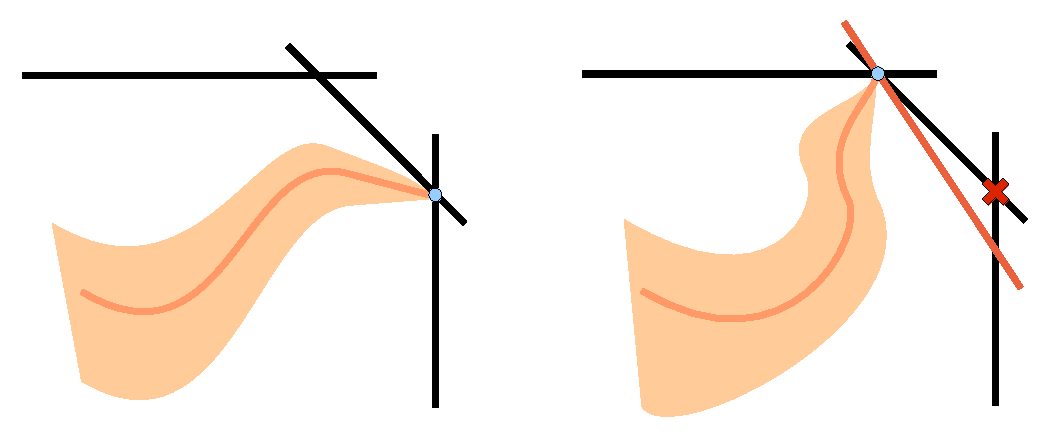
\includegraphics[scale=0.75]{figures/ws-path.eps}
\caption{Effect of a perturbation on the central path.}
\label{fig:ws-path}
\end{figure}

As presented in Chapter~\ref{ch:Ipm}, interior point methods approach 
the solution to the \KKT system of optimality conditions by relaxing 
the complementarity requirements and obtaining the perturbed
system (\ref{eq:PerturbedKKT}).
As moving towards a vertex can be interpreted as making 
a decision on the optimal partition, considering the 
system (\ref{eq:PerturbedKKT}) is equivalent to postponing 
the choice of the optimal partition.
If the vertex is not an 
optimal one, then the central path will not approach it.

The effectiveness of an interior point algorithm degrades when an 
iterate gets too close to a boundary before optimality is reached,
or, equivalently, when the iterate gets far from the central path.
In these situations the algorithm may spend many iterations in recovering
centrality, during which small steps are usually generated and thus
very slow progress is achieved (see Figure~\ref{fig:ws-behaviour}).

\begin{figure}[ht]
\centering
\vspace{-2ex}
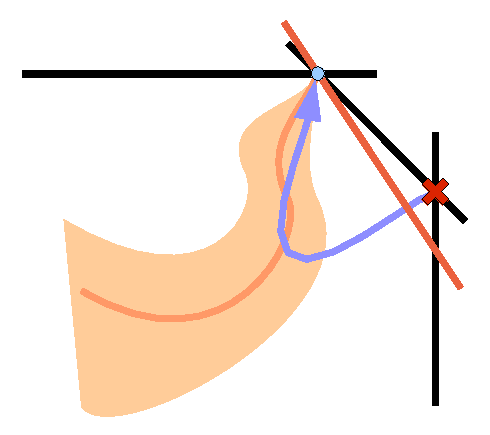
\includegraphics[scale=0.75]{figures/ws-behaviour.eps}
\caption{Typical behaviour of an interior point method if warm-started
         from the previously optimal solution.}
\label{fig:ws-behaviour}
\end{figure}

Hipolito \cite{Hipolito} considered the issue of robustness of 
search directions in interior point methods in these situations.
In his analysis, Hipolito showed that if the iterate is close 
to a boundary, the affine-scaling direction may be parallel to 
the nearby constraints. In such cases, the corrector direction 
may also display the same behaviour, and short stepsizes are 
obtained for the resulting combined search direction.
The analysis in \cite{Hipolito} concerns the
dual affine-scaling algorithm, but
it also seems to provide an interesting insight into the misbehaviour
of search directions used in primal--dual algorithms
when computed from non-central points.

The required features of a good warm-start candidate for an
interior point algorithm are somewhat contradictory.
The point should not be too close to the boundary of the feasible 
region in order to be able to absorb larger perturbations in the 
problem data. 
Also, it should be sufficiently advanced to provide 
computational savings over a cold-start iterate.
These considerations lead to the idea of storing an approximate
$\mu$-center well before reaching optimality 
\cite{Gondzio98,GondzioGrothey03,GondzioVial,YildirimWright}.

The theory and practice of warm-start techniques for interior point 
methods is a relatively new and still open field of study.
In the remainder of this section we present a review of some 
of the warm-start approaches proposed in the interior point literature.

%
%
\subsection{Literature review}

Mitchell \cite{phd:Mitchell} and Mitchell and Todd \cite{MitchellTodd}
analyse the potential reduction interior point method within
a cutting plane algorithm. They exploit the fact that
a primal feasible point can be constructed after a set of new
columns is added to the problem. They use this strategy with success
in a column generation scheme and more generally in the solution 
of combinatorial optimization problems.

The role of interior point methods in integer and combinatorial 
optimization has been comprehensively surveyed in \cite{Mitchell96} 
and \cite{MitchellPardalosResende98}. This is relevant as these classes
of optimization problems are generally solved by formulating a sequence
of linear relaxations, where the problem instances differ by the
addition of cutting planes and facet-inducing constraints.

Hipolito \cite{Hipolito} studies an alternative centering direction 
in the context of the dual affine-scaling algorithm. Such a 
direction is designed to move the iterate away from the boundary, 
overcoming the risk of moving parallel to it that was mentioned 
earlier in this section.
By considering a weighted least squares formulation, Hipolito 
develops the dual affine-scaling and the corresponding Newton 
centering directions. 
This study has an immediate interest for warm-starting approaches,
as the resulting direction points towards the interior of the 
feasible region, thus providing the algorithm with the necessary 
space to make fast progress. 
Unfortunately, it is developed only for the dual affine-scaling 
algorithm, and to the best of our knowledge there have been no 
studies on how to obtain a similar search direction in the 
primal--dual context.

Gondzio \cite{Gondzio98} presents a warm-start procedure for primal--dual
interior point methods in the context of a cutting plane method.
The interior point method is used to solve a sequence of restricted
master problems, which differ by one or more cutting planes.
By construction, in such a setting the solution to one problem
deeply violates some of the newly added constraints.
The optimal solution to a problem is necessarily very close 
to the boundary, thus is an unattractive starting point 
for a perturbed problem, and an alternative warm-start 
iterate needs to be defined.
The idea proposed in \cite{Gondzio98} is to store a nearly optimal 
point (3--4 digits of accuracy) to be employed as a warm-start point.
Because of the cutting plane setting, the problem is then solved to
optimality (7--8 digits of accuracy) in order to generate appropriate cuts.
As one requirement for a good iterate is centrality, it is of interest 
to perform a few centering steps on the stored iterate, the cost of 
which is marginal, as a factorisation is already available. The 
recentering steps proposed are based on
centrality correctors \cite{Gondzio96}.
An auxiliary feasibility recovery procedure may be needed as, due to 
the addition of cuts, large infeasibilities are often produced.

The warm-start approach proposed in \cite{Gondzio98} is extended
in \cite{GondzioVial} to the case of solving a sequence of problems 
with the same dimensions but changing problem data (the objective 
function or the right-hand side). Such situations arise 
in the context of decomposition approaches for large structured 
linear programs. 
In the case of Dantzig--Wolfe decomposition, successive subproblems 
differ only in the objective function, while in the case 
of Benders decomposition they differ only in the right-hand sides.
Following \cite{Gondzio98}, nearly optimal points are saved and used 
to warm-start the solution of subsequent subproblems \cite{GondzioVial}.

% An advanced application of this technique is studied in 
% \cite{GondzioVial}, where a decomposition approach for large 
% structured linear programs is implemented within an interior point 
% framework. In this setting, a sequence of linear problems is generated 
% by adding cutting planes to provide a polyhedral approximation of a 
% non-differentiable convex function, and a warm-start strategy is 
% applied when solving each subproblem.

\yildirim and Wright \cite{YildirimWright} consider again the case 
of solving a sequence of problems in fixed dimensions, and
analyse the number of iterations required to converge to a 
solution of the perturbed problem instance from the warm-start point.
They obtain worst-case estimates and
show that these estimates depend on the size of the perturbation 
as well as on the conditioning of the problem 
instances. Thus they obtain conditions under which the complexity 
of the warm-start approach is better than in the cold-start case.

The strategy proposed in \cite{YildirimWright} aims to absorb the 
primal and dual infeasibilities introduced by the perturbation in just 
one step.
% relying on the centrality of the iterate from one instance
% to provide enough centrality for the starting point of the next instance.
This strategy requires backtracking to an iterate for which $\mu$ is 
large enough to allow a full step for the correction direction they produce. 
The amount of necessary backtracking depends on the magnitude 
of the perturbation (as measured by the change in the problem data).
This is intuitively justified by considering that a large perturbation 
will produce a large adjustment. It is also essential to guarantee that 
a full step will not compromise the positivity requirements of the 
iterate.
%
To ensure the availability of an approximate $\mu$-center from which 
the perturbation can be absorbed in one step, a subset of 
iterates for different values of $\mu$ is stored.
When the size of the perturbation becomes known, the smallest $\mu$ 
that allows to absorb the perturbation
is retrieved, and the corresponding iterate is used as a 
warm-start point for the next problem in the sequence.
%
In \cite{YildirimWright}, two different corrections for the perturbation
are studied; one is based on least squares, the other on a Newton step 
correction.
A detailed computational comparison of these strategies has been 
carried out by John and \yildirim \cite{JohnYildirim}.

Gondzio and Grothey \cite{GondzioGrothey03} propose a different 
reoptimization technique for interior point methods.
As in \cite{YildirimWright}, they aim at obtaining conditions for 
perturbations that can be absorbed in one Newton step.
However, they measure perturbations by a relative measure of implied
primal and dual infeasibilities, and analyse recovery steps in
the primal and the dual spaces independently.

This reoptimization procedure is based on two phases. First, an attempt 
is made to absorb the infeasibilities caused by the perturbation with a full 
Newton step; second, the centrality of the iterate is improved. A
key feature of Gondzio and Grothey's approach \cite{GondzioGrothey03}
is that the primal search 
direction is governed only by the primal perturbation,
and the dual search direction only by the dual perturbation.
This corresponds to splitting the search direction into
two terms, $\Delta_1 w$ and $\Delta_2 w$, and solving
two independent Newton systems
%
\[
\left[ \begin{array}{ccc}
    A & 0 & 0 \\ 0 &A^T & I \\ S & 0 & X
  \end{array} \right]
\left[ \begin{array}{c}
    \Delta_1 x \\ \Delta_1 y \\ \Delta_1 s
  \end{array} \right] = 
\left[ \begin{array}{c}
    \xi_b \\ 0 \\ 0
  \end{array} \right],
\quad
\left[ \begin{array}{ccc}
    A & 0 & 0 \\ 0 &A^T & I \\ S & 0 & X
  \end{array} \right]
\left[ \begin{array}{c}
    \Delta_2 x \\ \Delta_2 y \\ \Delta_2 s
  \end{array} \right] = 
\left[ \begin{array}{c}
    0 \\ \xi_c \\ 0
  \end{array} \right].
\]
%
They produce bounds on the magnitude of primal residual $\xi_b$ 
and dual residual $\xi_c$ that can be absorbed in a single 
Newton step. Unlike to the results of \cite{YildirimWright}, 
the bounds of \cite{GondzioGrothey03} are easy to compute and 
thus can be used in practice.
If the residuals at the warm-start point do not satisfy these bounds,
a different iterate further 
away from optimality may be more likely to allow for a full Newton step.

A practical implementation is developed within an infeasible interior 
point method. In this context, a stronger emphasis may be put on 
reducing the infeasibilities. This is accomplished with additional 
centering steps.
An approximate $\mu$-center is stored for a tolerance level that 
depends on the magnitude of the expected perturbation. This does not 
exclude the possibility of storing a sequence of iterates, as proposed 
in \cite{YildirimWright}, thus postponing the choice of the one to 
use.
As the problem size does not change, an approximate $\mu$-center 
can immediately be used as an iterate for the next problem.
If only one iterate is stored, then the absorption of infeasibilities 
may be spread across a few iterations whenever the stepsizes fall 
below a predefined level.
As this strategy does not make assumptions upon the centrality of the 
warm-start iterate,
it can be initialised with any iterate.
Gondzio and Grothey \cite{GondzioGrothey03} apply this warm-start 
strategy successfully to structured problems for crash-start points that 
come from a cross-decomposition scheme, and thus may lack centrality.

A different approach has been studied by Benson and Shanno 
\cite{BensonShanno}. They investigate how to improve the efficiency 
of interior point methods in a reoptimization context by the use of 
a primal--dual penalty approach.
While standard penalty techniques are applied only in one space, 
the introduction of penalty parameters in both the primal and the 
dual problems allows the handling of perturbations in both spaces.
For example, an $l_1$ penalty can deal with changes in the right-hand
side of the constraints (primal changes), but has virtually no effect
on perturbations of the objective coefficients (dual changes).

Benson and Shanno's strategy relaxes the non-negativity constraints
for the decision
variables, penalising the violation in the objective, for both
the primal and dual problems.
The penalised problem allows the variables to become negative,
which provides more freedom of movement for the variables, with
the immediate advantage of allowing larger stepsizes along 
the computed search direction to be accepted. This favours faster progress
especially in the first few iterations, when the perturbation needs
to be absorbed.
Benson and Shanno \cite{BensonShanno} also provide some computational
evidence of the effectiveness of their strategy.

We will introduce a novel warm-start technique tailored to stochastic
linear programming in Chapter~\ref{ch:Warmstart}.
